\section{Sturm-Liouville Problems}

\noindent
In this section we consider eigenvalue problems of  the form
\begin{equation} \label{eq:13.2.1}
P_{0}(x)y''+P_{1}(x)y'+P_{2}(x)y+ \lambda R(x)y=0,\quad B_{1}(y)=0,\quad
B_{2}(y)=0,
\end{equation}
where
$$
B_{1}(y)=\alpha y(a)+\beta y'(a) \text{\quad and\quad}
B_{2}(y)=\rho y(b)+\delta y'(b).
$$
As in Section~13.1,  $\alpha$, $\beta$, $\rho$, and $\delta$
are real numbers, with
$$
\alpha^{2}+\beta^{2}>0\text{\;    and\; \;  } \rho^{2}+\delta^{2}>0,
$$
$P_{0}$, $P_{1}$, $P_{2}$, and $R$ are continuous, and $P_{0}$ and $R$
are positive on $[a,b]$.

We say that $\lambda$ is an \emph{eigenvalue} of  \eqref{eq:13.2.1} if
\eqref{eq:13.2.1} has a nontrivial solution $y$.   In this case, $y$ is an
\emph{eigenfunction associated with $\lambda$}, or
a $\lambda$-\emph{eigenfunction}.   \emph{Solving}  the eigenvalue
problem means finding all eigenvalues and associated eigenfunctions
of \eqref{eq:13.2.1}.

\begin{example}\label{example:13.2.1} \rm
Solve the eigenvalue problem
\begin{equation} \label{eq:13.2.2}
y'+3y'+2y+\lambda y=0,\quad  y(0)=0,\quad y(1)=0.
\end{equation}
\end{example}

\solution
The characteristic equation of \eqref{eq:13.2.2} is
$$
r^{2}+3r+2+\lambda=0,
$$
with zeros
$$
r_{1}=\frac{-3+\sqrt{1-4\lambda}}{2} \text{\quad   and \quad }
r_{2}=\frac{-3-\sqrt{1-4\lambda}}{2}.
$$
If $\lambda<1/4$ then  $r_{1}$ and $r_{2}$ are real and distinct, so the
general solution of the differential equation in  \eqref{eq:13.2.2} is
$$
y=c_{1}e^{r_{1}t}+c_{2}e^{r_{2}t}.
$$
The boundary conditions require that
\begin{eqnarray*}
c_{1}\phantom{e^{r_{1}}}+c_{2}\phantom{e^{r_{2}}}&=&0\\
c_{1}e^{r_{1}}+c_{2}e^{r_{2}}&=&0.
\end{eqnarray*}
Since the determinant of  this system is $e^{r_{2}}-e^{r_{1}}\ne0$, the
system has only the trivial solution. Therefore
$\lambda$ isn't  an eigenvalue of \eqref{eq:13.2.2}.

If $\lambda=1/4$ then $r_{1}=r_{2}=-3/2$, so the general solution of
\eqref{eq:13.2.2} is
$$
y=e^{-3x/2}(c_{1}+c_{2}x).
$$
The boundary condition $y(0)=0$ requires that $c_{1}=0$, so
$y=c_{2}xe^{-3x/2}$ and the boundary condition $y(0)$ requires that
$c_{2}=0$. Therefore $\lambda=1/4$  isn't  an eigenvalue of~\eqref{eq:13.2.2}.

If $\lambda>1/4$ then
$$
r_{1}=-\frac{3}{2}+i\omega \text{\quad   and\quad }
r_{2}=-\frac{3}{2}-i\omega,
$$
with
\begin{equation} \label{eq:13.2.3}
\omega =\frac{\sqrt{4\lambda-1}}{2}
\text{\quad  or, equivalently,\quad }  \lambda=\frac{1+4\omega^{2}}{4}.
\end{equation}
In this case the general solution of the differential equation in
\eqref{eq:13.2.2} is
$$
y=e^{-3x/2}(c_{1}\cos\omega x+c_{2}\sin\omega x).
$$
The boundary condition $y(0)=0$  requires that $c_{1}=0$, so
$y=c_{2}e^{-3x/2}\sin\omega x$, which holds with $c_{2}\ne0$ if and only if
$\omega=n\pi$, where $n$ is an integer. We may assume that $n$
is a positive integer. (Why?). From \eqref{eq:13.2.3}, the eigenvalues are
$\lambda_{n}=(1+4n^{2}\pi^{2})/4$, with associated eigenfunctions
$$
y_{n}=e^{-3x/2}\sin n\pi x,\quad  n=1,2,3,\dots.
$$

\begin{example} \label{example:13.2.2} \rm
Solve the eigenvalue problem
\begin{equation} \label{eq:13.2.4}
x^{2}y''+xy'+\lambda y=0,\quad y(1)=0,\quad y(2)=0.
\end{equation}
\end{example}

\solution
If  $\lambda=0$,  the differential equation in \eqref{eq:13.2.4}  reduces to
$x(xy')'=0$, so $xy'=c_{1}$,
$$
y'=\frac{c_{1}}{x}, \text{\quad and\quad}  y=c_{1}\ln x+c_{2}.
$$
The boundary condition $y(1)=0$ requires that $c_{2}=0$, so $y=c_{1}\ln x$.
The boundary condition  $y(2)=0$ requires that $c_{1}\ln2=0$, so $c_{1}=0$.
Therefore zero isn't  an eigenvalue of \eqref{eq:13.2.4}.

 If $\lambda<0$, we
write $\lambda=-k^{2}$ with $k>0$, so \eqref{eq:13.2.4} becomes
$$
x^{2}y''+xy'-k^{2}y=0,
$$
an Euler equation (Section~7.4) with indicial equation
$$
r^{2}-k^{2}=(r-k)(r+k)=0.
$$
Therefore
$$
y=c_{1}x^{k}+c_{2}x^{-k}.
$$
The boundary conditions require that
\begin{eqnarray*}
\phantom{2^{k}}c_{1}+\phantom{2^{-k}}c_{2}&=&0 \\
2^{k}c_{1}+2^{-k}c_{2}&=&0.
\end{eqnarray*}
Since the determinant of this system  is $2^{-k}-2^{k}\ne0$,
$c_{1}=c_{2}=0$. Therefore \eqref{eq:13.2.4} has no negative eigenvalues.

If $\lambda>0$ we write $\lambda=k^{2}$ with $k>0$. Then  \eqref{eq:13.2.4}
becomes
$$
x^{2}y''+xy' +k^{2}y=0,
$$
an Euler equation with indicial equation
$$
r^{2}+k^{2}=(r-ik)(r+ik)=0,
$$
so
$$
y=c_{1}\cos(k\ln x)+c_{2}\sin(k\ln x).
$$
 The boundary condition $y(1)=0$
requires that $c_{1}=0$. Therefore $y=c_{2}\sin(k\ln x)$. This holds with
$c_{2}\ne0$ if and only if $k=n\pi/\ln 2$, where $n$ is a positive integer.
Hence, the eigenvalues of \eqref{eq:13.2.4} are $\lambda_{n}=(n\pi/\ln2)^{2}$,
with associated eigenfunctions
$$
y_{n}=\sin\left(\frac{n\pi}{\ln2}\ln x\right),\quad n=1,2,3,\dots.
$$

For theoretical purposes, it's useful to rewrite the differential equation
in \eqref{eq:13.2.1} in a different form, provided by the next theorem.

\begin{theorem}\color{blue} \label{thmtype:13.2.1}
If $P_{0}$, $P_{1}$, $P_{2}$, and $R$ are continuous and $P_{0}$ and $R$
are positive on a closed interval $[a,b]$, then the equation
\begin{equation} \label{eq:13.2.5}
P_{0}(x)y''+P_{1}(x)y'+P_{2}(x)y+\lambda R(x)y=0
\end{equation}
can be rewritten as
\begin{equation} \label{eq:13.2.6}
(p(x)y')'+q(x)y+\lambda r(x)y=0,
\end{equation}
where $p$, $p'$, $q$ and $r$ are continuous and $p$ and $r$ are positive
on $[a,b]$.
\end{theorem}

\proof
We begin by rewriting \eqref{eq:13.2.5} as
\begin{equation} \label{eq:13.2.7}
y''+u(x)y'+v(x)y+\lambda R_{1}(x)y=0,
\end{equation}
with $u=P_{1}/P_{0}$, $v=P_{2}/P_{0}$, and $R_{1}=R/P_{0}$. (Note that
$R_{1}$ is positive on $[a,b]$.)  Now let $p(x)=e^{U(x)}$, where $U$ is any
antiderivative of $u$. Then $p$ is positive  on  $[a,b]$ and, since
$U'=u$,
\begin{equation} \label{eq:13.2.8}
p'(x)=p(x)u(x)
\end{equation}
is continuous on $[a,b]$. Multiplying \eqref{eq:13.2.7} by $p(x)$  yields
\begin{equation} \label{eq:13.2.9}
p(x)y''+p(x)u(x)y'+p(x)v(x)y+\lambda p(x)R_{1}(x)y=0.
\end{equation}
Since $p$ is positive on $[a,b]$, this equation has the same solutions as
\eqref{eq:13.2.5}. From \eqref{eq:13.2.8},
$$
(p(x)y')'=p(x)y''+p'(x)y'=p(x)y''+p(x)u(x)y',
$$
so \eqref{eq:13.2.9} can be rewritten as in \eqref{eq:13.2.6}, with $q(x)=p(x)v(x)$
and $r(x)=p(x)R_{1}(x)$. This completes the proof.

It is to be understood throughout the rest of this section that $p$, $q$,
and $r$ have the properties stated in Theorem~\ref{thmtype:13.2.1}. Moreover,
whenever we write $Ly$ in a general statement, we mean
$$
Ly=(p(x)y')'+q(x)y.
$$

The differential equation \eqref{eq:13.2.6} is called a
\href{https://mathshistory.st-andrews.ac.uk/Biographies/Sturm/}
{\color{blue}\it Sturm}--\href{https://mathshistory.st-andrews.ac.uk/Biographies/Liouville/}
{\color{blue}\it Liouville  equation}, and the
eigenvalue problem
\begin{equation} \label{eq:13.2.10}
(p(x)y')'+q(x)y+\lambda r(x)y=0,\quad B_{1}(y)=0,\quad
B_{2}(y)=0,
\end{equation}
which is equivalent to \eqref{eq:13.2.1}, is called a
\href{https://mathshistory.st-andrews.ac.uk/Biographies/Sturm/}
{\color{blue}\it Sturm-Liouville
problem}.

\begin{example}\label{example:13.2.3} \rm
Rewrite the eigenvalue problem
\begin{equation} \label{eq:13.2.11}
y''+3y'+(2+\lambda)y=0,\quad y(0)=0,\quad y(1)=0
\end{equation}
of Example~\ref{example:13.2.1}  as a Sturm-Liouville problem.
\end{example}

\solution
Comparing \eqref{eq:13.2.11} to \eqref{eq:13.2.7}  shows that $u(x)=3$, so we   take
$U(x)=3x$ and $p(x)=e^{3x}$. Multiplying the differential equation in
\eqref{eq:13.2.11} by $e^{3x}$ yields
$$
e^{3x}(y''+3y')+2e^{3x}y+\lambda e^{3x}y=0.
$$
Since
$$
e^{3x}(y''+3y')=(e^{3x}y')',
$$
 \eqref{eq:13.2.11} is equivalent to the Sturm--Liouville problem
\begin{equation} \label{eq:13.2.12}
(e^{3x}y')'+2e^{3x}y+\lambda e^{3x}y=0,\quad y(0)=0,\quad y(1)=0.
\end{equation}

\begin{example}\label{example:13.2.4} \rm
Rewrite the eigenvalue problem
\begin{equation} \label{eq:13.2.13}
x^{2}y''+xy'+\lambda y=0,\quad y(1)=0,\quad y(2)=0
\end{equation}
of Example~\ref{example:13.2.2}  as a Sturm-Liouville problem.
\end{example}

\solution
Dividing the differential equation in \eqref{eq:13.2.13} by $x^{2}$  yields
$$
y''+\frac{1}{x}y'+\frac{\lambda}{x^{2}}y=0.
$$
Comparing this to \eqref{eq:13.2.7} shows that $u(x)=1/x$, so we take $U(x)=\ln
x$ and $p(x)=e^{\ln x}=x$.
Multiplying the differential equation by $x$ yields
$$
xy''+y'+\frac{\lambda}{x}y=0.
$$
Since
$$
xy''+y'=(xy')',
$$
\eqref{eq:13.2.13} is equivalent to the Sturm--Liouville problem
\begin{equation} \label{eq:13.2.14}
(xy')'+\frac{\lambda}{x}y=0,\quad y(1)=0,\quad y(2)=0.
\end{equation} \bbox

Problems 1--4 of Section~11.1  are Sturm--Liouville problems.
(Problem~5 isn't , although some authors use a definition of
\href{https://mathshistory.st-andrews.ac.uk/Biographies/Sturm/}
{\color{blue}\it Sturm-Liouville problem}
that does include it.)  We were able to find
the eigenvalues of Problems 1-4  explicitly because in each problem the
coefficients in the boundary conditions satisfy $\alpha\beta=0$ and
$\rho\delta=0$; that is, each boundary condition  involves either $y$
or $y'$, but not both. If this isn't true then the eigenvalues can't in
general be expressed exactly by simple formulas;     rather, approximate
values
must be obtained by numerical solution of equations derived by requiring
the determinants of certain $2\times 2$ systems of homogeneous equations to
be zero. To apply the numerical methods effectively, graphical methods
must be used to determine approximate locations of the zeros of these
determinants. Then the zeros can be computed accurately by
numerical methods.

\begin{example}  \label{example:13.2.5} \rm
Solve the Sturm--Liouville problem
\begin{equation} \label{eq:13.2.15}
y''+\lambda y=0, \quad y(0)+y'(0)=0,\quad y(1)+3y'(1)=0.
\end{equation}
\end{example}

\solution  If
$\lambda=0$, the differential equation in \eqref{eq:13.2.15} reduces
to $y''=0$, with general solution $y=c_{1}+c_{2}x$. The boundary conditions
require that
\begin{eqnarray*}
c_{1}+\phantom{4}c_{2}&=&0\\
c_{1}+4c_{2}&=&0,
\end{eqnarray*}
so $c_{1}=c_{2}=0$. Therefore zero isn't  an eigenvalue of \eqref{eq:13.2.15}.

If $\lambda<0$,  we write
$\lambda=-k^{2}$ where $k>0$, and the differential equation in
\eqref{eq:13.2.15}   becomes $y''-k^{2}y=0$, with general solution
\begin{equation} \label{eq:13.2.16}
y=c_{1}\cosh kx+c_{2}\sinh kx,
\end{equation}
so
$$
y'=k(c_{1}\sinh kx+c_{2}\cosh kx).
$$
The boundary conditions require that
\begin{equation} \label{eq:13.2.17}
\begin{gathered}
c_{1}+kc_{2}=0\\
(\cosh k+3k\sinh k)c_{1}+(\sinh k+3k\cosh k)c_{2}=0.
\end{gathered}
\end{equation}
The determinant of this system is
\begin{eqnarray*}
D_{N}(k)&=&
\left|\begin{array}{cccccc}
1&k\\
\cosh k+3k\sinh k&\sinh k+3k \cosh k
\end{array}\right|      \\
&=& (1-3k^{2})\sinh k+2k \cosh k.
\end{eqnarray*}
Therefore the  system \eqref{eq:13.2.17} has a nontrivial solution if and only
if
$D_{N}(k)=0$ or, equivalently,
\begin{equation} \label{eq:13.2.18}
\tanh k=-\frac{2k}{1-3k^{2}}.
\end{equation}
The graph of the right side (Figure~\ref{figure:13.2.1}) has a vertical
asymptote at
$k=1/\sqrt{3}$.
Since the two sides have different signs if $k<1/\sqrt{3}$,  this equation
has no solution in $(0,1/\sqrt{3})$. Figure~\ref{figure:13.2.1} shows the
graphs
of the two sides of \eqref{eq:13.2.18} on an interval to the right of the
vertical asymptote, which is indicated by the dashed line. You can see that
the two curves intersect near $k_{0}=1.2$, Given this estimate, you can use
Newton's to compute $k_{0}$  more accurately. We computed $k_{0}\approx
1.1219395$. Therefore $-k_{0}^{2}\approx -1.2587483$ is an eigenvalue of
\eqref{eq:13.2.15}. From \eqref{eq:13.2.16} and the first equation in \eqref{eq:13.2.17},
$$
y_{0}=k_{0}\cosh k_{0}x-\sinh k_{0}x.
$$

\begin{figure}[tbp]
  \centering\color{blue}
  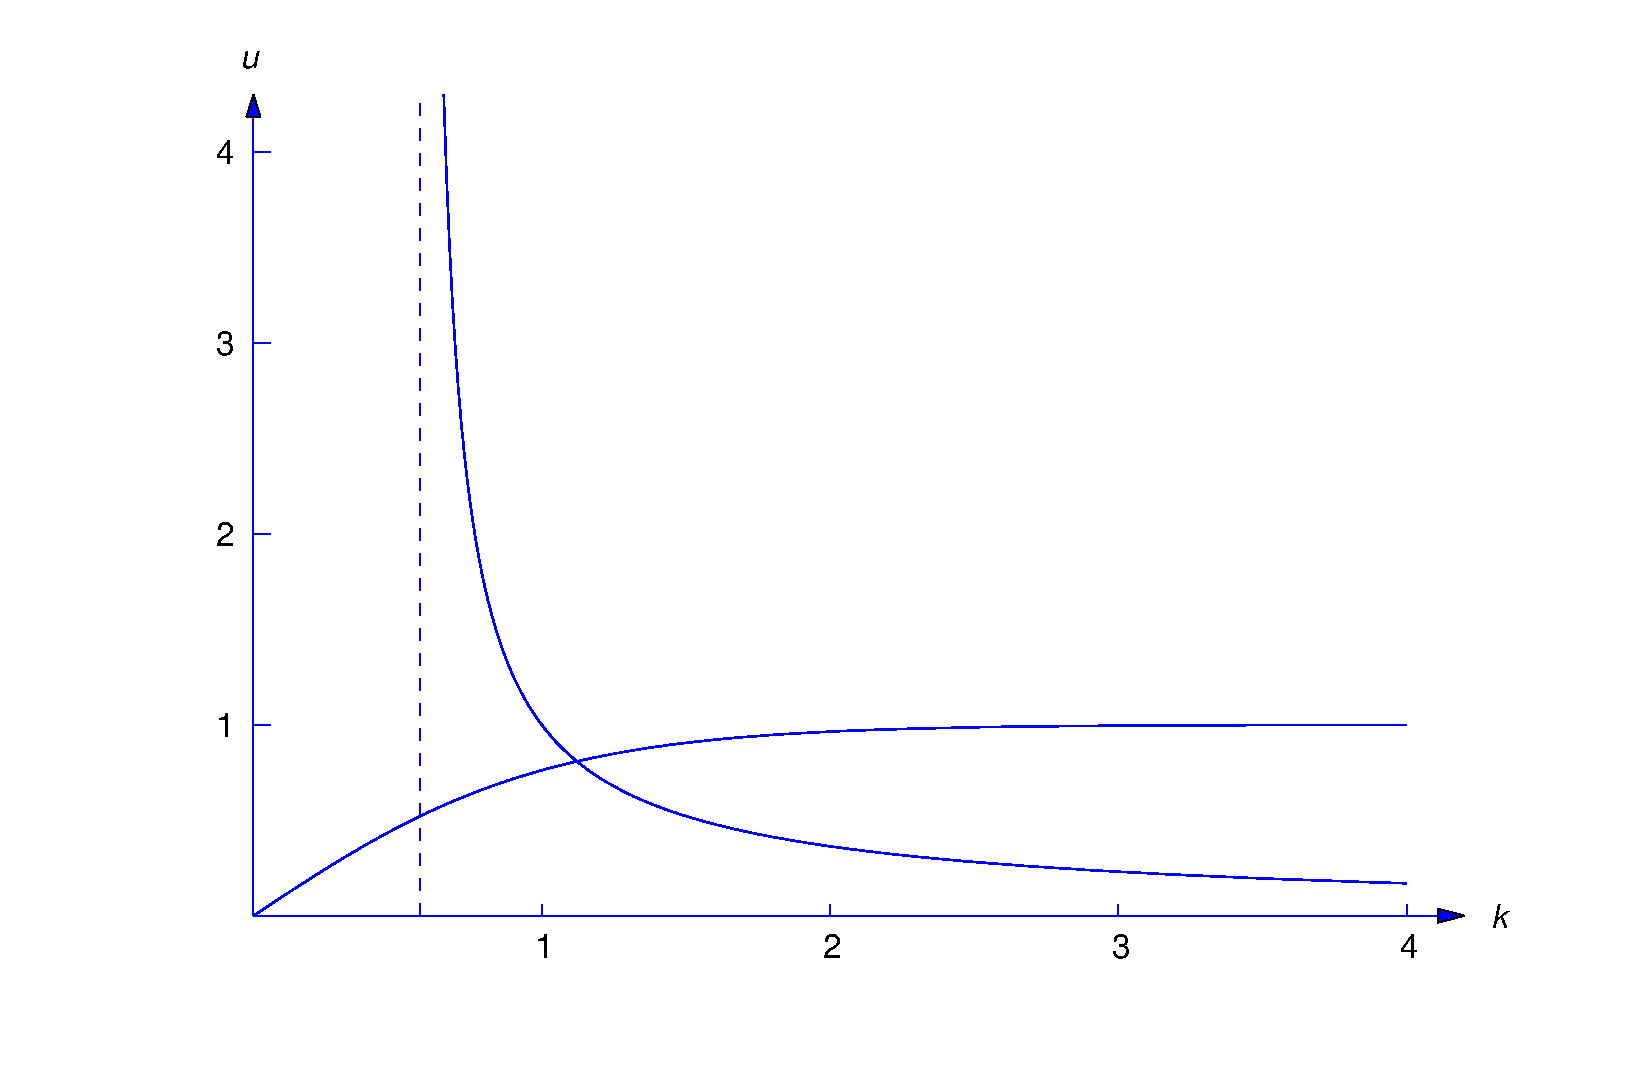
\includegraphics[bb=-78 148 689 643,width=5.67in,height=3.66in,keepaspectratio]{fig130201}
\caption{$u=\tanh k$  and $u=-2k/(1-3k^2)$}
  \label{figure:13.2.1}
\end{figure}

If $\lambda>0$ we write
$\lambda=k^{2}$ where $k>0$, and   differential equation in
\eqref{eq:13.2.15} becomes $y''+k^{2}y=0$, with general solution
\begin{equation} \label{eq:13.2.19}
y= \cos kx + c_{2}\sin kx,
\end{equation}
so
$$
y'=k(-c_{1}\sin kx+c_{2}\cos kx).
$$
The boundary conditions require that
\begin{equation} \label{eq:13.2.20}
\begin{gathered}
c_{1}+kc_{2}=0\\
(\cos k-3k\sin k)c_{1}+(\sin k+3k\cos k)c_{2}=0.
\end{gathered}
\end{equation}
The determinant of this system is
\begin{eqnarray*}
D_{P}(k)&=&
\left|\begin{array}{cccccc}
1&k\\
\cos k-3k\sin k&\sin k+3k \cos k
\end{array}\right|      \\
&=& (1+3k^{2})\sin k+2k \cos k.
\end{eqnarray*}
The system \eqref{eq:13.2.20}  has a nontrivial solution if and only if
$D_{P}(k)=0$ or, equivalently,
$$
\tan k=-\frac{2k}{1+3k^{2}}.
$$
Figure~\ref{figure:13.2.2} shows  the graphs of the two sides of this
equation.
You can see from the figure that  the graphs intersect at infinitely many
points
$k_{n}\approx n\pi$ ($n=1$, $2$, $3$,\dots), where the error in this
approximation approaches zero as $n\to\infty$. Given this estimate, you can
use Newton's method to compute $k_{n}$  more accurately. We computed
\begin{eqnarray*}
k_{1}&\approx&\phantom{1}2.9256856,\\
k_{2}&\approx&\phantom{1} 6.1765914,\\
k_{3}&\approx&\phantom{1} 9.3538959,\\
k_{4}&\approx& 12.5132570.
\end{eqnarray*}
The estimates of the corresponding eigenvalues $\lambda_{n}=k_{n}^{2}$ are
\begin{eqnarray*}
\lambda_{1}&\approx&\phantom{15} 8.5596361,\\
\lambda_{2}&\approx&\phantom{5} 38.1502809,\\
\lambda_{3}&\approx&\phantom{5} 87.4953676,\\
\lambda_{4}&\approx& 156.5815998.
\end{eqnarray*}
From \eqref{eq:13.2.19}   and the first equation in \eqref{eq:13.2.20},
$$
y_{n}=k_{n}\cos k_{n}x-\sin k_{n}x
$$
is an eigenfunction associated with $\lambda_{n}$  \bbox

\begin{figure}[tbp]
  \centering\color{blue}
  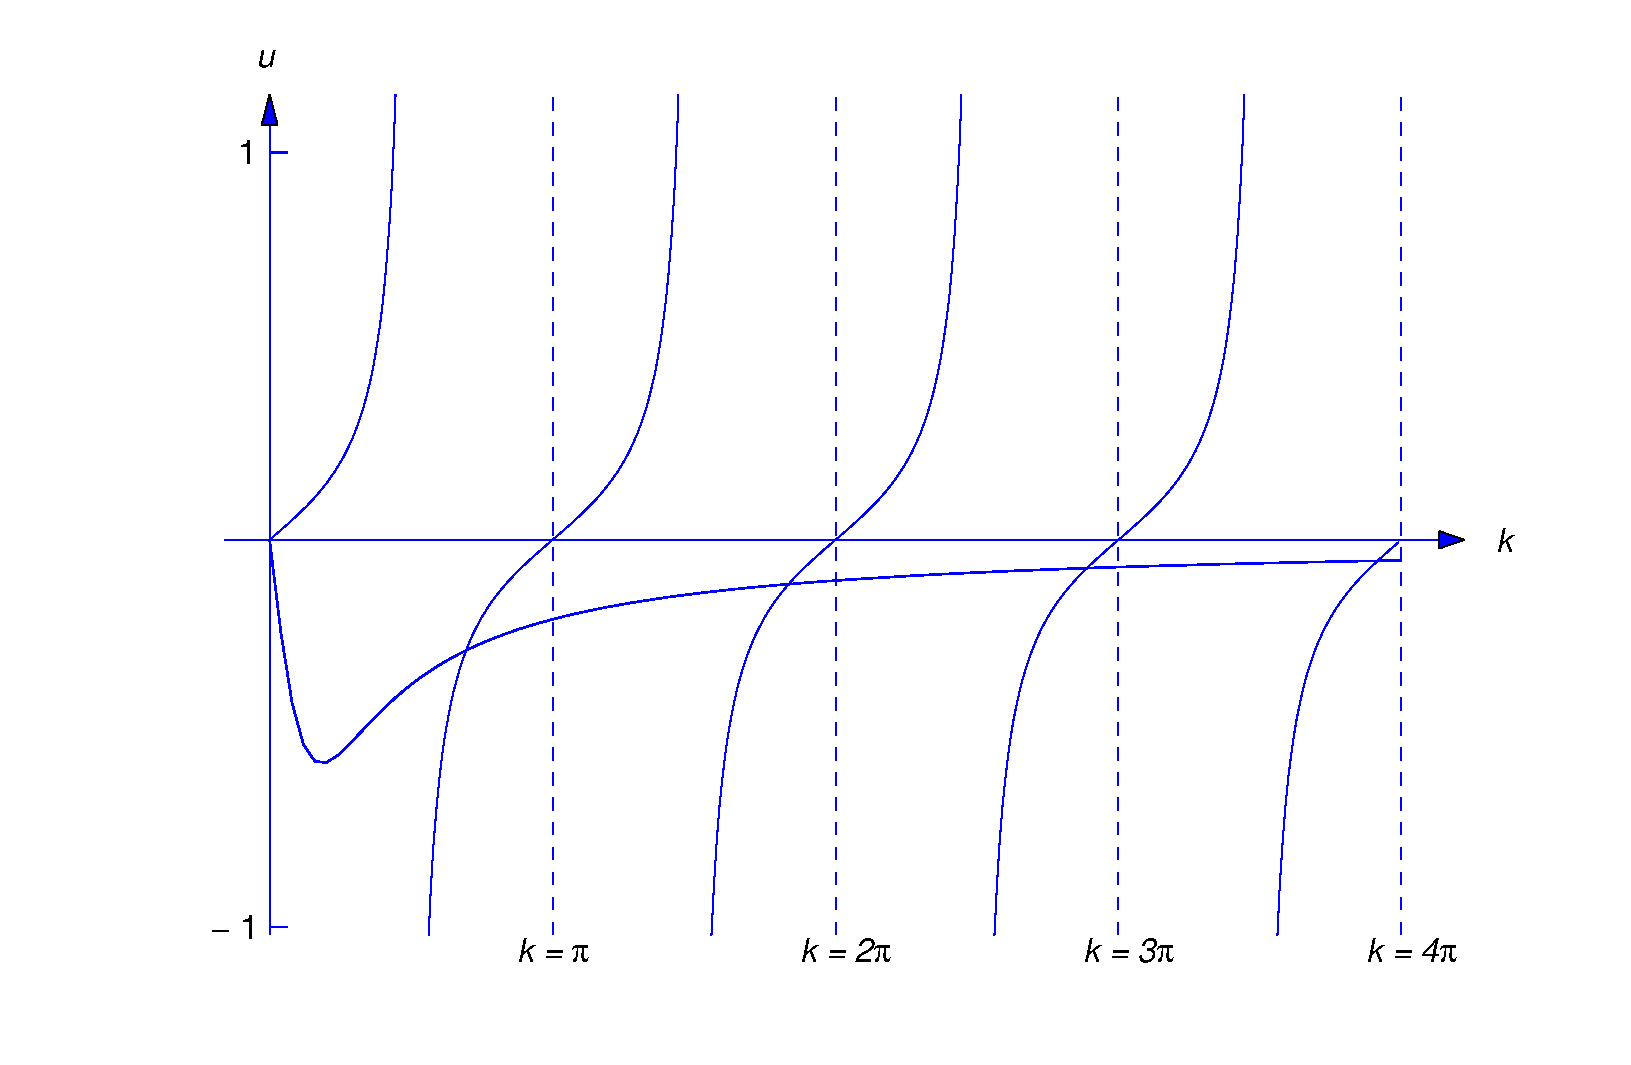
\includegraphics[bb=-78 148 689 643,width=5.67in,height=3.66in,keepaspectratio]{fig130202}
\caption{$u=\tan k$ and $u=-2k/(1+k)$}
  \label{figure:13.2.2}
\end{figure}

Since the differential equations in \eqref{eq:13.2.12} and \eqref{eq:13.2.14}
are more complicated than those in \eqref{eq:13.2.11} and \eqref{eq:13.2.13}
respectively, what is the point of Theorem~\ref{thmtype:13.2.1}?
The point is this: to solve a \emph{specific} problem, it may be better
to deal with it directly, as we did in Examples~\ref{example:13.2.1}
and \ref{example:13.2.2};     however, we'll see that transforming the
\emph{general} eigenvalue problem \eqref{eq:13.2.1} to the Sturm--Liouville
problem \eqref{eq:13.2.10}  leads to results applicable to \emph{all}
eigenvalue problems of the form \eqref{eq:13.2.1}.

\begin{theorem}\color{blue} \label{thmtype:13.2.2}
If
$$
Ly=(p(x)y')'+q(x)y
$$
and $u$ and $v$  are twice continuously  functions on $[a,b]$ that satisfy
the boundary conditions $B_{1}(y)=0$ and $B_{2}(y)=0$,  then
\begin{equation} \label{eq:13.2.21}
\int_{a}^{b}[u(x)Lv(x)-v(x)Lu(x)]\,dx=0.
\end{equation}
\end{theorem}

\proof
Integration by parts yields
\begin{eqnarray*}
\int_{a}^{b}[u(x)Lv(x)-v(x)Lu(x)]\,dx&=&
\int_{a}^{b}[u(x)(p(x)v'(x))'-v(x)(p(x)u'(x))']\,dx\\
&=& p(x)[u(x)v'(x)-u'(x)v(x)]\bigg|_{a}^{b}\\
&&-\int_{a}^{b}p(x)[u'(x)v'(x)-u'(x)v'(x)]\,dx.
\end{eqnarray*}
Since the last integral equals zero,
\begin{equation} \label{eq:13.2.22}
\int_{a}^{b}[u(x)Lv(x)-v(x)Lu(x)]\,dx =
 p(x)[u(x)v'(x)-u'(x)v'(x)]\bigg|_{a}^{b}.
\end{equation}
By assumption, $B_{1}(u)=B_{1}(v)=0$ and $B_{2}(u)=B_{2}(v)=0$. Therefore
$$
\begin{aligned}
\alpha u(a)+\beta u'(a)&=0\\
\alpha v(a)+\beta v'(a)&=0\\
\end{aligned}
\quad \text{\quad   and\quad}\quad
\begin{gathered}
\rho u(b)+\delta u'(b)=0\phantom{.}\\
\rho v(b)+\delta v'(b)=0.
\end{gathered}
$$
Since $\alpha^{2}+\beta^{2}>0$ and $\rho^{2}+\delta^{2}>0$, the
determinants of these two systems must both be zero; that is,
$$
u(a)v'(a)-u'(a)v(a)=u(b)v'(b)-u'(b)v(b)=0.
$$
This and \eqref{eq:13.2.22} imply \eqref{eq:13.2.21}, which completes the
proof.

The next theorem shows that a Sturm--Liouville problem has no complex
eigenvalues.

\begin{theorem}\color{blue} \label{thmtype:13.2.3}
If $\lambda=p+qi$ with $q\ne0$  then the boundary value problem
$$
Ly+\lambda r(x)y=0,\quad B_{1}(y)=0,\quad B_{2}(y)=0
$$
has only the trivial solution.
\end{theorem}

\proof For this theorem to make sense, we must consider complex-valued
solutions  of
\begin{equation} \label{eq:13.2.23}
Ly+(p+iq)r(x,y)y=0.
\end{equation}
If $y=u+iv$ where $u$ and $v$ are real-valued and twice differentiable,
we define $y'=u'+iv'$ and $y''=u''+iv''$. We say that $y$  is a solution of
\eqref{eq:13.2.23} if
the   real and imaginary parts of the left side of \eqref{eq:13.2.23} are both
zero.  Since $Ly=(p(x)'y)'+q(x)y$  and $p$, $q$, and $r$ are real-valued,
\begin{eqnarray*}
Ly+\lambda
r(x)y&=&L(u+iv)+(p+iq)r(x)(u+iv)\\
&=&Lu+r(x)(pu-qv)+i[Lv+r(x)(pu+qv)],
\end{eqnarray*}
so $Ly+\lambda r(x)y=0$ if and only if
\begin{eqnarray*}
Lu+r(x)(pu-qv)&=&0\\
Lv+r(x)(qu+pv)&=&0.
\end{eqnarray*}
Multiplying the first equation by $v$ and the second by $u$  yields
\begin{eqnarray*}
vLu+r(x)(puv-qv^{2})&=&0\\
uLv+r(x)(qu^{2}+puv)&=&0.
\end{eqnarray*}
Subtracting the first equation from the second yields
$$
uLv-vLu+qr(x)(u^{2}+v^{2})=0,
$$
so
\begin{equation} \label{eq:13.2.24}
\int_{a}^{b}[u(x)Lv(x)-v(x)Lu(x)]\,dx+
\int_{a}^{b}r(x)[u^{2}(x)+v^{2}(x)]\,dx=0.
\end{equation}
Since
$$
B_{1}(y)=B_{1}(u+iv)=B_{1}(u)+iB_{1}(v)
$$
and
$$
B_{2}(y)=B_{2}(u+iv)=B_{2}(u)+iB_{2}(v),
$$
$B_{1}(y)=0$ and $B_{2}(y)=0$  implies that
$$
B_{1}(u)=B_{2}(u)=B_{1}(v)=B_{2}(v)=0.
$$
 Therefore Theorem~\ref{thmtype:13.2.2}
implies that  first integral in
\eqref{eq:13.2.24} equals zero, so \eqref{eq:13.2.24} reduces to
$$
q\int_{a}^{b}r(x)[u^{2}(x)+v^{2}(x)]\,dx =0.
$$
Since $r$ is positive on $[a,b]$  and $q\ne0$ by assumption, this implies
that $u\equiv0$ and $v\equiv0$ on $[a,b]$. Therefore $y\equiv0$ on
$[a,b]$, which completes the proof.

\begin{theorem}\color{blue} \label{thmtype:13.2.4}
If $\lambda_{1}$ and $\lambda_{2}$ are distinct eigenvalues of the
Sturm--Liouville  problem
\begin{equation} \label{eq:13.2.25}
Ly+\lambda r(x)y=0,\quad B_{1}(y)=0,\quad B_{2}(y)=0
\end{equation}
with associated eigenfunctions $u$ and $v$ respectively, then
\begin{equation} \label{eq:13.2.26}
\int_{a}^{b}r(x)u(x)v(x)\,dx=0.
\end{equation}
\end{theorem}

\proof Since $u$ and $v$ satisfy the boundary conditions in \eqref{eq:13.2.25},
Theorem~\ref{thmtype:13.2.2} implies that
$$
\int_{a}^{b}[u(x)Lv(x)-v(x)Lu(x)]\,dx=0.
$$
Since $Lu=-\lambda_{1}ru$ and $Lv=-\lambda_{2}rv$, this implies that
$$
(\lambda_{1}-\lambda_{2})\int_{a}^{b}r(x)u(x)v(x)\,dx=0.
$$
Since $\lambda_{1}\ne\lambda_{2}$, this implies \eqref{eq:13.2.26}, which
completes the proof.

If $u$  and $v$ are any integrable functions on $[a,b]$ and
$$
\int_{a}^{b} r(x)u(x)v(x)\,dx=0,
$$
we say that $u$ and $v$ \emph{orthogonal on} $[a,b]$
 \emph{with respect to} $r=r(x)$.

Theorem~\ref{thmtype:13.1.1}  implies the next theorem.

\begin{theorem}\color{blue} \label{thmtype:13.2.5}
If $u\not\equiv0$ and $v$ both satisfy
$$
Ly+\lambda r(x)y=0,\quad B_{1}(y)=0,\quad B_{2}(y)=0,
$$
then $v=cu$ for some constant $c$.
\end{theorem}

We've now proved parts of the next theorem. A complete proof is
beyond the scope of this book.

\begin{theorem}\color{blue} \label{thmtype:13.2.6}
The set of all eigenvalues of the Sturm--Liouville problem
$$
Ly+\lambda r(x)y=0,\quad B_{1}(y)=0,\quad B_{2}(y)=0
$$
can be ordered as
$$
\lambda_{1}<\lambda_{2}<\cdots<\lambda_{n}<\cdots,
$$
and
$$
\lim_{n\to\infty} \lambda_{n}=\infty.
$$
For each $n$,  if $y_{n}$ is an arbitrary $\lambda_{n}$-eigenfunction,
then every $\lambda_{n}$-eigenfunction is a constant multiple of $y_{n}$.
If $m\ne n$,   $y_{m}$ and $y_{n}$  are orthogonal $[a,b]$  with
respect to  $r=r(x)$;    that is,
\begin{equation} \label{eq:13.2.27}
\int_{a}^{b} r(x)y_{m}(x)y_{n}(x)\,dx=0.
\end{equation}
\end{theorem}

 You may want to verify \eqref{eq:13.2.27} for the eigenfunctions obtained in
Examples~\ref{example:13.2.1}  and \ref{example:13.2.2}.

In conclusion, we mention the next theorem. The proof is beyond the
scope of this book.

\begin{theorem}\color{blue} \label{thmtype:13.2.7}
Let $\lambda_{1}<\lambda_{2}<\cdots<\lambda_{n}<\cdots$  be the eigenvalues
of the Sturm--Liouville problem
$$
Ly+\lambda r(x)y=0,\quad B_{1}(y)=0,\quad B_{2}(y)=0,
$$
with associated eigenvectors $y_{1}$,  $y_{2}$, \dots, $y_{n}$, \dots.
 Suppose $f$  is piecewise smooth
$($Definition~$\ref{thmtype:11.2.3})$ on $[a,b]$.  For each $n$, let
$$
c_{n}=\frac{\dst{\int_{a}^{b}}r(x)f(x)y_{n}(x)\,dx}
{\dst{\int_{a}^{b}}r(x)y_{n}^{2}(x)\,dx}.
$$
Then
$$
\frac{f(x-)+f(x+)}{2}=\sum_{n=1}^{\infty}c_{n}y_{n}(x)
$$
for all $x$ in the open interval $(a,b)$.
\end{theorem}

\exercises

\emph{In Exercises~$\ref{exer:13.2.1}$--$\ref{exer:13.2.7}$  rewrite the equation
in Sturm--Liouville form $($with $\lambda=0)$. Assume that $b$, $c$,
$\alpha$, and $\nu$ are constants.}

\begin{exerciselist}

\item\label{exer:13.2.1} $y''+by'+cy=0$

\item\label{exer:13.2.2} $x^{2}y''+xy'+(x^{2}-\nu^{2})y=0$ \quad (Bessel's
equation)

\item\label{exer:13.2.3} $(1-x^{2})y''-xy'+\alpha^{2}y=0$ \quad
(Chebyshev's equation)

\item\label{exer:13.2.4} $x^{2}y''+bxy'+cy=0$ \quad (Euler's equation)

\item\label{exer:13.2.5} $y''-2xy'+2\alpha y=0$ \quad (Hermite's equation)
\item\label{exer:13.2.6} $xy''+(1-x)y'+\alpha y=0$ \quad (Laguerre's equation)

\item\label{exer:13.2.7} $(1-x^{2})y''-2xy'+\alpha(\alpha+1)y=0$
\quad (Legendre's equation)

\item\label{exer:13.2.8}
In Example~\ref{example:13.2.4} we found that the eigenvalue problem
\begin{equation}
x^{2}y''+xy'+\lambda y=0,\quad y(1)=0,\quad y(2)=0 \tag{A}
\end{equation}
is equivalent to the Sturm-Liouville problem
\begin{equation} \tag{B}
(xy')'+\frac{\lambda}{x}y=0,\quad y(1)=0,\quad y(2)=0.
\end{equation}
Multiply the differential equation in (B) by $y$ and integrate to show that
$$
\lambda\int_{1}^{2}\frac{y^{2}(x)}{x}\,dx=\int_{1}^{2}x(y'(x))^{2}\,dx.
$$
Conclude from this that the eigenvalues of (A) are all positive.

\item\label{exer:13.2.9}
Solve the eigenvalue problem
$$
y''+2y'+y+\lambda y=0,\quad y(0)=0, \quad y(1)=0.
$$

\item\label{exer:13.2.10}
Solve the eigenvalue problem
$$
y''+2y'+y+\lambda y=0,\quad y'(0)=0, \quad y'(1)=0.
$$

\exercisetext{
In Exercises~$\ref{exer:13.2.11}$--$\ref{exer:13.2.20}$:
\part{a} Determine whether $\lambda=0$ is an eigenvalue. If it is, find an
 associated eigenfunction.

\part{b}  Compute the negative eigenvalues with  errors not greater than
$5\times 10^{-8}$.  State the form of the associated eigenfunctions.

\part{c}  Compute the first four positive eigenvalues with  errors not
greater than
$5\times 10^{-8.}$  State the form of the associated eigenfunctions.}

 \item\label{exer:13.2.11} \Cex
$y''+\lambda y=0$, \quad  $y(0)+2y'(0)=0$,\quad $y(2)=0$

 \item\label{exer:13.2.12} \Cex
$y''+\lambda y=0$, \quad  $y'(0)=0$,\quad $y(1)-2y'(1)=0$

\item\label{exer:13.2.13}\Cex
$y''+\lambda y=0$, \quad  $y(0)-y'(0)=0$,\quad $y'(\pi)=0$

 \item\label{exer:13.2.14}\Cex
$y''+\lambda y=0$, \quad  $y(0)+2y'(0)=0$,\quad $y(\pi)=0$

\item\label{exer:13.2.15}  \Cex
$y''+\lambda y=0$, \quad  $y'(0)=0$,\quad $y(2)-y'(2)=0$

 \item\label{exer:13.2.16} \Cex
$y''+\lambda y=0$, \quad  $y(0)+y'(0)=0$,\quad $y(2)+2y'(2)=0$

 \item\label{exer:13.2.17} \Cex
$y''+\lambda y=0$, \quad  $y(0)+2y'(0)=0$,\quad $y(3)-2y'(3)=0$

 \item\label{exer:13.2.18} \Cex
$y''+\lambda y=0$, \quad  $3y(0)+y'(0)=0$,\quad $3y(2)-2y'(2)=0$

 \item\label{exer:13.2.19} \Cex
$y''+\lambda y=0$, \quad  $y(0)+2y'(0)=0$,\quad $y(3)-y'(3)=0$

 \item\label{exer:13.2.20}  \Cex
$y''+\lambda y=0$, \quad  $5y(0)+2y'(0)=0$,\quad $5y(1)-2y'(1)=0$

\item\label{exer:13.2.21}
Find the first five eigenvalues of  the boundary value problem
$$
y''+2y'+y+\lambda y=0,\quad y(0)=0,\quad y'(1)=0
$$
with errors not greater than $5\times 10^{-8}$. State the form of the
associated eigenfunctions.

\exercisetext{In Exercises~\ref{exer:13.2.22}--\ref{exer:13.2.24} take it as given
that
$\{xe^{kx},xe^{-kx}\}$ and $\{x\cos kx, x\sin kx\}$ are fundamental sets of
solutions of
$$
x^{2}y''-2xy'+2y-k^{2}x^{2}y=0
$$
and
$$
x^{2}y''-2xy'+2y+k^{2}x^{2}y=0,
$$
respectively.}

\item\label{exer:13.2.22}
Solve the eigenvalue problem  for

$$
x^{2}y''-2xy'+2y+\lambda x^{2}y=0, \quad y(1)=0,\quad y(2)=0.
$$

\item\label{exer:13.2.23} \Cex
Find the first five eigenvalues of
$$
x^{2}y''-2xy'+2y+\lambda x^{2}y=0, \quad y'(1)=0,\quad y(2)=0
$$
with errors no greater than $5\times 10^{-8}$. State the form of the
associated eigenfunctions.

\item\label{exer:13.2.24}  \Cex
Find the first five eigenvalues of
$$
x^{2}y''-2xy'+2y+\lambda x^{2}y=0, \quad y(1)=0,\quad y'(2)=0
$$
with errors no greater than $5\times 10^{-8}$. State the form of the
associated eigenfunctions.

\item\label{exer:13.2.25}
Consider the Sturm-Liouville problem
\begin{equation}   \tag{A}
y''+\lambda y=0,\quad y(0)=0,\quad y(L)+\delta y'(L)=0.
\end{equation}

\part{a} Show that (A)  can't have more than one negative eigenvalue,
and find the values of $\delta$ for which it has one.

\part{b} Find all values of $\delta$ such that $\lambda=0$ is an eigenvalue
of (A).

\part{c} Show that $\lambda=k^{2}$ with $k>0$ is an eigenvalue of (A)
if and only if
\begin{equation} \tag{B}
\tan kL=-\delta k.
\end{equation}

\part{d}
For
 $n=1$, $2$, \dots, let $y_{n}$  be an eigenfunction  associated with
$\lambda_{n}=k_{n}^{2}$. From Theorem~\ref{thmtype:13.2.4}, $y_{m}$  and
$y_{n}$ are orthogonal over $[0,L]$ if $m\ne n$. Verify this  directly.
\hint{Integrate by parts twice and use} (B).

\item\label{exer:13.2.26}
Solve the Sturm-Liouville problem
$$
y''+\lambda y=0,\quad y(0)+\alpha y'(0)=0,\quad y(\pi)+\alpha y'(\pi)=0,
$$
where $\alpha\ne0$.

\item\label{exer:13.2.27}\Lex
Consider the Sturm-Liouville problem
\begin{equation}   \tag{A}
y''+\lambda y=0,\quad y(0)+\alpha y'(0)=0,\quad y(1)+(\alpha-1) y'(1)=0,
\end{equation}
where $0<\alpha<1$.

\part{a} Show that $\lambda=0$  is an eigenvalue of   (A),
and find an associated eigenfunction.

\part{b} Show that  (A)   has a negative eigenvalue,
and find the form of an associated eigenfunction.

\part{c}   Give a graphical argument to show that (A) has infinitely many
positive eigenvalues $\lambda_{1} < \lambda_{2}<\cdots
<\lambda_{n}<\cdots$, and state the form of the associated eigenfunctions.

\exercisetext{
Exercises~\ref{exer:13.2.28}--\ref{exer:13.2.30}  deal with the Sturm--Liouville
problem
\begin{equation} \tag{SL}
y''+\lambda y=0,\quad \alpha y(0)+\beta y'(0),\quad
\rho y(L)+\delta y'(L)=0,
\end{equation}
where $\alpha^{2}+\beta^{2}>0$  and  $\rho^{2}+\delta^{2}>0$.}

\item\label{exer:13.2.28}
Show that $\lambda=0$ is an eigenvalue of (SL)  if and only if
$$
\alpha(\rho L+\delta)-\beta\rho =0.
$$

\item\label{exer:13.2.29} \Lex
The point of this exercise is that (SL) can't have more than two negative
eigenvalues.

\part{a} Show that $\lambda$ is a negative eigenvalue of (SL)
if and only if $\lambda=-k^{2}$, where $k$  is a positive solution of
$$
(\alpha\rho-\beta\delta k^{2})\sinh kL+k(\alpha\delta-\beta\rho)\cosh kL.
$$

\part{b}  Suppose $\alpha\delta-\beta\rho=0$.  Show that (SL)
has a negative eigenvalue if and only if $\alpha\rho$ and $\beta\delta$
are both nonzero. Find the negative eigenvalue and an associated
eigenfunction. \hint{Show that in this case $\rho=p\alpha$ and
$s=q\beta$, where $q\ne0$.}

\part{c}  Suppose $\beta\rho-\alpha\delta\ne0$. We know from
Section~11.1 that (SL) has no negative eigenvalues
if $\alpha\rho=0$ and $\beta\delta=0$. Assume that either $\alpha\rho\ne0$
or $\beta\delta\ne0$. Then we can rewrite (A) as
$$
\tanh kL=
\frac{k(\beta\rho-\alpha\delta)}{\alpha\rho-\beta\delta k^{2}}.
$$
By graphing both sides of this equation on the same axes (there are
several possibilities for the right side), show that it has at most
two positive solutions, so (SL) has at most two negative eigenvalues.

\item\label{exer:13.2.30} \Lex
The point of this exercise is that (SL) has infinitely many positive
eigenvalues $\lambda_{1}<\lambda_{2}<\cdots<\lambda_{n}<\cdots$, and
that $\lim_{n\to\infty}\lambda_{n}=\infty$.

\part{a} Show that $\lambda$ is a positive eigenvalue of (SL)
if and only if $\lambda=k^{2}$, where $k$ is a positive solution of
\begin{equation} \tag{A}
(\alpha\rho+\beta\delta k^{2})\sin kL+k(\alpha\delta-\beta\rho)\cos kL=0.
\end{equation}

\part{b} Suppose $\alpha\delta-\beta\rho=0$. Show that the positive
eigenvalues
 of (SL) are $\lambda_{n}=(n\pi/L)^{2}$, $n=1$, $2$, $3$, \dots.
\hint{Recall the hint in Exercise~\ref{exer:13.2.29}\part{b}.}

Now suppose $\alpha\delta-\beta\rho\ne0$. From
Section~11.1,  if $\alpha\rho=0$ and $\beta\delta=0$,
then (SL) has the eigenvalues
$$
\lambda_{n}=[(2n-1)\pi/2L]^{2},\quad  n=1,2,3, \dots
$$
(why?), so let's suppose  in addition that at least one of the products
$\alpha\rho$ and $\beta\delta$ is nonzero.  Then we can rewrite (A)
as
\begin{equation} \tag{B}
\tan kL=
\frac{k(\beta\rho-\alpha\delta)}
{\alpha\rho-\beta\delta k^{2}}.
\end{equation}
By graphing both sides of this equation on the same axes
(there are several possibilities for the right side), convince yourself of
the following:

\part{c} If $\beta\delta=0$, there's a positive integer $N$ such that (B)
has one solution $k_{n}$ in each of the intervals
\begin{equation} \tag{C}
\left((2n-1)\pi/L, (2n+1)\pi/L)\right),\quad n=N,N+1,N+2,\dots,
\end{equation}
and either
$$
\lim_{n\to\infty}\left(k_{n}-\frac{(2n-1)\pi}{2L}\right) =0
\text{\quad or\quad}
\lim_{n\to\infty}\left(k_{n}-\frac{(2n+1)\pi}{2L}\right)=0.
$$

\part{d}
If $\beta\delta\ne0$, there's a positive integer $N$  such that (B) has
one solution $k_{n}$ in each of the intervals (C) and
$$
\lim_{n\to\infty}\left(k_{n}-\frac{n\pi}{N}\right)=0.
$$

\item\label{exer:13.2.31}
The following Sturm--Liouville problems are generalizations of Problems
1--4 of Section~11.1.

\quad  Problem 1:   \quad $(p(x)y')'+\lambda r(x)y=0$,\quad
$y(a)=0$,\quad  $y(b)=0$

\quad  Problem 2:   \quad $(p(x)y')'+\lambda r(x)y=0$,\quad
$y'(a)=0$,\quad  $y'(b)=0$

\quad  Problem 3:   \quad $(p(x)y')'+\lambda r(x)y=0$,\quad
$y(a)=0$,\quad  $y'(b)=0$

\quad Problem 4:   \quad $(p(x)y')'+\lambda r(x)y=0$,\quad
$y'(a)=0$,\quad  $y(b)=0$

Prove: Problems~1--4  have no negative eigenvalues. Moreover, $\lambda=0$
is an eigenvalue of Problem~2 with associated eigenfunction $y_{0}=1$,
but $\lambda=0$ isn't  an eigenvalue of Problems 1, 3, and 4.
\hint{See the proof of Theorem~\ref{thmtype:11.1.1}.}

\item\label{exer:13.2.32} Show that the eigenvalues of the Sturm--Liouville
problem
$$
(p(x)y')'+\lambda r(x)y=0,\quad \alpha y(a)+ \beta y'(a)=0,\quad
\rho y(b)+\delta y'(b)
$$
are all positive if $\alpha\beta\le 0$, \,  $\rho\delta\ge 0$, and
$(\alpha\beta)^{2}+(\rho\delta)^{2}>0$.

\end{exerciselist}

